\chapter{Hyperparameters}
\label{app:hparams}

\tabref{tab:app-hparams} lists every setting used to train and evaluate the models in this thesis. Settings not listed are the defaults of the code base and are recorded in the notebooks.

\begin{table}[htbp]
    \centering
    \caption{Training, model and evaluation hyperparameters.}
    \label{tab:app-hparams}
    \footnotesize\renewcommand{\arraystretch}{0.95}
    \begin{tabularx}{\textwidth}{@{}l >{\raggedright\arraybackslash}X@{}}
        \toprule
        Setting & Value \\
        \midrule
        \multicolumn{2}{@{}l}{\textit{Model}} \\
        Neuron & Deterministic LIF, $\tau = 2$, $V_\mathrm{th} = 0.5$, hard reset, detached reset \\
        Surrogate gradient & $\alpha / (2(1 + \alpha|x|)^2)$, $\alpha = 4$ \\
        Encoding & Direct (image repeated at every timestep), per-channel normalisation \\
        Maximum horizon & $T_{\max} = 8$ \\
        Stochastic / Parseval / weight perturbation & Disabled \\
        \addlinespace
        \multicolumn{2}{@{}l}{\textit{Training}} \\
        Epochs & 100 \\
        Optimiser & SGD, momentum 0.9, weight decay $10^{-4}$ \\
        Learning rate & 0.1, 5-epoch linear warm-up, cosine decay \\
        Batch size & 256 \\
        Precision & Automatic mixed precision (float16), gradient clipping at norm 1.0 \\
        Augmentation & Random crop (padding 4), horizontal flip, Cutout ($1 \times 16$ px) \\
        Clean regime & 100\% clean images \\
        Adversarial regime & 100\% RFGSM images, $\epsilon = \alpha = 8/255$, random start $\pm 0.1\epsilon$ \\
        Timestep schedule & Fixed-T8: $T = 8$; mixed-T: $T \sim \mathcal{U}\{1, \dots, 8\}$ per batch \\
        Checkpoint selection & Best clean validation accuracy at $T = 8$, evaluated every 5 epochs \\
        Seeds & 0 (single-run models); 0, 1, 2 (multi-seed) \\
        \addlinespace
        \multicolumn{2}{@{}l}{\textit{Evaluation}} \\
        Splits & 40{,}000 train / 5{,}000 validation / 5{,}000 calibration / 10{,}000 test \\
        Fixed horizons & $T \in \{1, \dots, 8\}$ \\
        VT thresholds & $\theta \in \{0.5, 0.6, 0.7, 0.8, 0.85, 0.9, 0.95, 0.99\}$ \\
        Compute matching & Nearest mean SynOps, sample-exact VT accounting \\
        VT-neutral tolerance & $\delta = 1$ (primary); 0.5 and 2 (sensitivity) \\
        Temperature (temperature softmax) & 2 \\
        \addlinespace
        \multicolumn{2}{@{}l}{\textit{Attacks}} \\
        Budget & $\ell_\infty$, $\epsilon = 8/255$ \\
        PGD-20 & 20 steps, step size $2/255$, uniform random start, CE loss on exit-step logits \\
        AutoAttack & Standard version (APGD-CE, APGD-T, FAB-T, Square), attack seed 0 \\
        Exit handling & Full 8-step trace; loss on accumulated logits at the deployed exit step \\
        Wrong early exit & Eq.~\eqref{eq:wrong-exit}, confidence weight $\lambda_c = 0.25$ \\
        Compute overuse & Eq.~\eqref{eq:overuse}, label-preservation weight $\lambda_p = 1$ \\
        Attack subset & Class-balanced; 2{,}000 (single run), 1{,}000 (multi-seed), seed 0 \\
        \bottomrule
    \end{tabularx}
\end{table}

\chapter{Additional Results}
\label{app:tables}

This appendix collects the full result tables from which the figures and summary tables of \chapref{ch:results} are drawn. All tables are generated from the raw result files by \texttt{analysis/make\_tables.py}.

\begin{figure}[htbp]
    \centering
    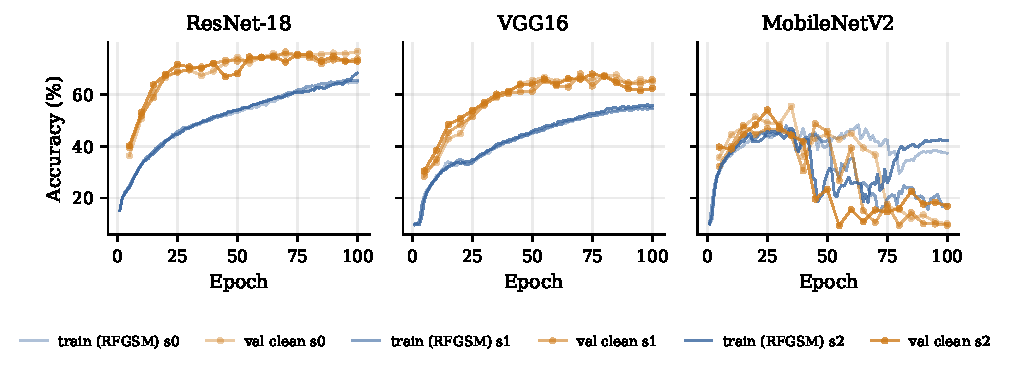
\includegraphics[width=\textwidth]{train_curves}
    \caption[Training curves of the multi-seed adversarially trained models]{Training curves of the multi-seed adversarially trained models: RFGSM training accuracy (blue, every epoch) and clean validation accuracy at $T = 8$ (orange, every five epochs) for seeds 0--2. MobileNetV2 training is unstable, and one seed's training accuracy collapses after about epoch 40.}
    \label{fig:train-curves}
\end{figure}

\begin{table}[htbp]
\centering
\caption[SynOps of fixed-timestep inference]{Mean SynOps per image ($10^6$) of fixed-timestep inference at each horizon (test set).}
\label{tab:app-fixed-synops}
\footnotesize
\begin{tabular}{@{}l rrrrrrrr@{}}
\toprule
Configuration & $T{=}1$ & 2 & 3 & 4 & 5 & 6 & 7 & 8 \\
\midrule
R18 clean & 17.1 & 78.7 & 127.0 & 191.8 & 237.3 & 304.7 & 349.5 & 413.7 \\
R18 adv (1) & 22.1 & 65.2 & 112.0 & 156.9 & 196.1 & 246.9 & 285.7 & 333.3 \\
R18 adv (2) & 10.6 & 56.5 & 89.9 & 138.6 & 164.1 & 218.9 & 240.9 & 292.6 \\
R18 clean mixT & 42.2 & 122.0 & 191.3 & 270.0 & 338.9 & 418.9 & 487.0 & 565.0 \\
R18 adv mixT & 33.2 & 90.9 & 144.4 & 200.7 & 254.2 & 312.2 & 364.4 & 420.4 \\
VGG clean & 4.3 & 28.5 & 51.3 & 81.4 & 100.9 & 132.5 & 151.4 & 182.3 \\
VGG adv & 4.5 & 20.4 & 38.1 & 59.0 & 73.9 & 96.5 & 110.9 & 133.3 \\
MBv2 clean & 45.3 & 92.3 & 139.4 & 187.7 & 234.0 & 282.6 & 328.7 & 377.0 \\
MBv2 adv & 45.9 & 96.2 & 146.4 & 196.9 & 245.4 & 296.7 & 345.0 & 395.8 \\
\bottomrule
\end{tabular}
\end{table}

\begin{table}[htbp]
\centering
\caption{VT sweep for R18 clean (test set, max-softmax rule).}
\label{tab:app-vt-r18_clean_T8}
\footnotesize
\begin{tabular}{@{}c r r r@{}}
\toprule
$\theta$ & Accuracy (\%) & Mean depth & SynOps ($10^6$) \\
\midrule
0.50 & 86.53 & 2.12 & 84.7 \\
0.60 & 87.72 & 2.24 & 90.9 \\
0.70 & 88.91 & 2.39 & 99.4 \\
0.80 & 89.80 & 2.62 & 111.4 \\
0.85 & 90.13 & 2.79 & 120.7 \\
0.90 & 90.62 & 3.01 & 133.0 \\
0.95 & 90.96 & 3.37 & 152.6 \\
0.99 & 91.26 & 4.22 & 199.4 \\
\bottomrule
\end{tabular}
\end{table}

\begin{table}[htbp]
\centering
\caption{VT sweep for R18 adv (1) (test set, max-softmax rule).}
\label{tab:app-vt-r18_adv_T8}
\footnotesize
\begin{tabular}{@{}c r r r@{}}
\toprule
$\theta$ & Accuracy (\%) & Mean depth & SynOps ($10^6$) \\
\midrule
0.50 & 71.48 & 4.33 & 163.3 \\
0.60 & 72.83 & 5.01 & 193.3 \\
0.70 & 73.49 & 5.58 & 219.2 \\
0.80 & 73.66 & 6.11 & 243.4 \\
0.85 & 73.69 & 6.40 & 256.4 \\
0.90 & 73.73 & 6.71 & 271.2 \\
0.95 & 73.73 & 7.10 & 289.2 \\
0.99 & 73.73 & 7.61 & 314.0 \\
\bottomrule
\end{tabular}
\end{table}

\begin{table}[htbp]
\centering
\caption{VT sweep for R18 adv (2) (test set, max-softmax rule).}
\label{tab:app-vt-r18_adv_T8_rep}
\footnotesize
\begin{tabular}{@{}c r r r@{}}
\toprule
$\theta$ & Accuracy (\%) & Mean depth & SynOps ($10^6$) \\
\midrule
0.50 & 75.15 & 4.54 & 151.6 \\
0.60 & 76.42 & 5.13 & 174.7 \\
0.70 & 76.83 & 5.62 & 194.2 \\
0.80 & 77.13 & 6.14 & 215.2 \\
0.85 & 77.16 & 6.41 & 226.0 \\
0.90 & 77.20 & 6.73 & 239.0 \\
0.95 & 77.19 & 7.14 & 255.9 \\
0.99 & 77.19 & 7.69 & 279.0 \\
\bottomrule
\end{tabular}
\end{table}

\begin{table}[htbp]
\centering
\caption{VT sweep for R18 clean mixT (test set, max-softmax rule).}
\label{tab:app-vt-r18_clean_mixT}
\footnotesize
\begin{tabular}{@{}c r r r@{}}
\toprule
$\theta$ & Accuracy (\%) & Mean depth & SynOps ($10^6$) \\
\midrule
0.50 & 52.47 & 1.20 & 58.1 \\
0.60 & 59.63 & 1.38 & 72.0 \\
0.70 & 66.26 & 1.63 & 91.0 \\
0.80 & 72.90 & 1.98 & 117.4 \\
0.85 & 76.39 & 2.23 & 136.1 \\
0.90 & 80.03 & 2.57 & 161.1 \\
0.95 & 84.15 & 3.12 & 201.7 \\
0.99 & 88.92 & 4.24 & 284.8 \\
\bottomrule
\end{tabular}
\end{table}

\begin{table}[htbp]
\centering
\caption{VT sweep for R18 adv mixT (test set, max-softmax rule).}
\label{tab:app-vt-r18_adv_mixT}
\footnotesize
\begin{tabular}{@{}c r r r@{}}
\toprule
$\theta$ & Accuracy (\%) & Mean depth & SynOps ($10^6$) \\
\midrule
0.50 & 70.60 & 3.16 & 146.8 \\
0.60 & 74.70 & 3.98 & 191.1 \\
0.70 & 76.47 & 4.73 & 231.8 \\
0.80 & 77.50 & 5.43 & 270.7 \\
0.85 & 77.63 & 5.78 & 290.3 \\
0.90 & 77.74 & 6.18 & 313.0 \\
0.95 & 77.75 & 6.70 & 342.9 \\
0.99 & 77.75 & 7.42 & 385.1 \\
\bottomrule
\end{tabular}
\end{table}

\begin{table}[htbp]
\centering
\caption{VT sweep for VGG clean (test set, max-softmax rule).}
\label{tab:app-vt-vgg_clean_T8}
\footnotesize
\begin{tabular}{@{}c r r r@{}}
\toprule
$\theta$ & Accuracy (\%) & Mean depth & SynOps ($10^6$) \\
\midrule
0.50 & 84.16 & 2.89 & 49.2 \\
0.60 & 85.78 & 3.20 & 57.1 \\
0.70 & 86.99 & 3.53 & 65.2 \\
0.80 & 87.75 & 3.89 & 74.1 \\
0.85 & 87.94 & 4.08 & 78.9 \\
0.90 & 88.08 & 4.33 & 85.2 \\
0.95 & 88.14 & 4.68 & 94.2 \\
0.99 & 88.18 & 5.46 & 114.3 \\
\bottomrule
\end{tabular}
\end{table}

\begin{table}[htbp]
\centering
\caption{VT sweep for VGG adv (test set, max-softmax rule).}
\label{tab:app-vt-vgg_adv_T8}
\footnotesize
\begin{tabular}{@{}c r r r@{}}
\toprule
$\theta$ & Accuracy (\%) & Mean depth & SynOps ($10^6$) \\
\midrule
0.50 & 64.64 & 5.74 & 86.6 \\
0.60 & 65.21 & 6.27 & 97.0 \\
0.70 & 65.41 & 6.69 & 105.3 \\
0.80 & 65.49 & 7.05 & 112.6 \\
0.85 & 65.48 & 7.21 & 115.9 \\
0.90 & 65.49 & 7.39 & 119.6 \\
0.95 & 65.49 & 7.60 & 124.2 \\
0.99 & 65.49 & 7.87 & 130.2 \\
\bottomrule
\end{tabular}
\end{table}

\begin{table}[htbp]
\centering
\caption{VT sweep for MBv2 clean (test set, max-softmax rule).}
\label{tab:app-vt-mbv2_clean_T8}
\footnotesize
\begin{tabular}{@{}c r r r@{}}
\toprule
$\theta$ & Accuracy (\%) & Mean depth & SynOps ($10^6$) \\
\midrule
0.50 & 28.96 & 2.38 & 110.4 \\
0.60 & 39.32 & 2.95 & 137.6 \\
0.70 & 49.96 & 3.67 & 171.7 \\
0.80 & 60.53 & 4.61 & 216.0 \\
0.85 & 66.50 & 5.17 & 242.9 \\
0.90 & 71.33 & 5.80 & 272.7 \\
0.95 & 75.68 & 6.56 & 308.6 \\
0.99 & 78.08 & 7.41 & 349.2 \\
\bottomrule
\end{tabular}
\end{table}

\begin{table}[htbp]
\centering
\caption{VT sweep for MBv2 adv (test set, max-softmax rule).}
\label{tab:app-vt-mbv2_adv_T8}
\footnotesize
\begin{tabular}{@{}c r r r@{}}
\toprule
$\theta$ & Accuracy (\%) & Mean depth & SynOps ($10^6$) \\
\midrule
0.50 & 49.65 & 6.55 & 323.2 \\
0.60 & 50.92 & 7.21 & 356.2 \\
0.70 & 51.38 & 7.62 & 377.0 \\
0.80 & 51.48 & 7.86 & 388.9 \\
0.85 & 51.49 & 7.93 & 392.3 \\
0.90 & 51.49 & 7.97 & 394.5 \\
0.95 & 51.49 & 8.00 & 395.6 \\
0.99 & 51.49 & 8.00 & 395.8 \\
\bottomrule
\end{tabular}
\end{table}

\begin{table}[htbp]
\centering
\caption[Compute at the VT-neutral operating points]{Compute at the VT-neutral operating points ($\delta = 1$, test set). Mismatch: VT SynOps relative to the matched control. CI: binomial 95\% half-width of the VT accuracy.}
\label{tab:app-neutral-synops}
\footnotesize
\begin{tabular}{@{}l c r c r r r r@{}}
\toprule
Configuration & $\theta$ & VT SynOps & $T^*$ & Matched SynOps & Mismatch & $T{=}8$ SynOps & CI \\
\midrule
R18 clean & 0.90 & 133.0 & 3 & 127.0 & +4.7\% & 413.7 & $\pm$0.57 \\
R18 adv (1) & 0.60 & 193.3 & 5 & 196.1 & -1.5\% & 333.3 & $\pm$0.87 \\
R18 adv (2) & 0.60 & 174.7 & 5 & 164.1 & +6.5\% & 292.6 & $\pm$0.83 \\
R18 clean mixT & 0.99 & 284.8 & 4 & 270.0 & +5.5\% & 565.0 & $\pm$0.62 \\
R18 adv mixT & 0.80 & 270.7 & 5 & 254.2 & +6.5\% & 420.4 & $\pm$0.82 \\
VGG clean & 0.80 & 74.1 & 4 & 81.4 & -8.9\% & 182.3 & $\pm$0.64 \\
VGG adv & 0.50 & 86.6 & 6 & 96.5 & -10.2\% & 133.3 & $\pm$0.94 \\
MBv2 clean & 0.99 & 349.2 & 7 & 328.7 & +6.2\% & 377.0 & $\pm$0.81 \\
MBv2 adv & 0.60 & 356.2 & 7 & 345.0 & +3.2\% & 395.8 & $\pm$0.98 \\
\bottomrule
\end{tabular}
\end{table}

\begin{table}[htbp]
\centering
\caption[Stopping rules at degenerate reference depths]{Stopping-rule results for the two configurations whose reference depth came from a degenerate max-gain operating point (test set).}
\label{tab:app-stoprules-degenerate}
\footnotesize
\begin{tabular}{@{}l l r r@{}}
\toprule
Configuration & Rule & Accuracy (\%) & Mean depth \\
\midrule
R18 clean mixT & fixed T8 baseline & 90.57 & 8.00 \\
R18 clean mixT & max softmax & 59.63 & 1.38 \\
R18 clean mixT & margin & 65.36 & 1.62 \\
R18 clean mixT & entropy & 55.87 & 1.26 \\
R18 clean mixT & temperature softmax & 72.24 & 1.84 \\
R18 clean mixT & evidential surrogate & 45.15 & 1.05 \\
\addlinespace
MBv2 clean & fixed T8 baseline & 77.66 & 8.00 \\
MBv2 clean & max softmax & 28.96 & 2.38 \\
MBv2 clean & margin & 48.82 & 3.58 \\
MBv2 clean & entropy & 29.92 & 2.45 \\
MBv2 clean & temperature softmax & 57.05 & 4.29 \\
MBv2 clean & evidential surrogate & 18.10 & 2.00 \\
\bottomrule
\end{tabular}
\end{table}

{\footnotesize\setlength{\tabcolsep}{3pt}
\begin{longtable}{@{}l l c l l l r r r@{}}
\caption[All single-run attack results]{All single-run attack results, including the neighbouring thresholds of each attacked VT operating point. The run-1 adversarial ResNet-18 is omitted (see \secref{sec:res-threats}).}\label{tab:app-attacks}\\
\toprule
Configuration & Mode & $\theta$ & Role & Attack & Objective & Acc. & Depth & $n$ \\
\midrule
\endfirsthead
\toprule
Configuration & Mode & $\theta$ & Role & Attack & Objective & Acc. & Depth & $n$ \\
\midrule
\endhead
R18 clean & fixed & --- & fixed T8 baseline & pgd & untargeted & 0.00 & 8.00 & 10000 \\
R18 clean & vt & 0.60 & lower neighbor & pgd & untargeted & 0.00 & 2.00 & 10000 \\
R18 clean & vt & 0.70 & selected & pgd & untargeted & 0.02 & 2.00 & 10000 \\
R18 clean & vt & 0.80 & upper neighbor & pgd & untargeted & 0.00 & 2.01 & 10000 \\
R18 clean & vt & 0.60 & lower neighbor & pgd & wrong early exit & 0.00 & 2.00 & 10000 \\
R18 clean & vt & 0.70 & selected & pgd & wrong early exit & 0.00 & 2.00 & 10000 \\
R18 clean & vt & 0.80 & upper neighbor & pgd & wrong early exit & 0.00 & 2.00 & 10000 \\
R18 clean & vt & 0.60 & lower neighbor & pgd & compute overuse & 59.74 & 3.09 & 10000 \\
R18 clean & vt & 0.70 & selected & pgd & compute overuse & 60.58 & 3.58 & 10000 \\
R18 clean & vt & 0.80 & upper neighbor & pgd & compute overuse & 63.10 & 4.23 & 10000 \\
R18 clean & fixed & --- & fixed T8 baseline & autoattack & untargeted & 0.06 & 8.00 & 10000 \\
R18 clean & vt & 0.70 & selected & autoattack & untargeted & 0.02 & 2.14 & 10000 \\
\addlinespace
R18 adv (2) & fixed & --- & fixed T8 baseline & pgd & untargeted & 46.10 & 8.00 & 2000 \\
R18 adv (2) & vt & 0.50 & lower neighbor & pgd & untargeted & 47.75 & 5.13 & 2000 \\
R18 adv (2) & vt & 0.60 & selected & pgd & untargeted & 48.70 & 5.86 & 2000 \\
R18 adv (2) & vt & 0.70 & upper neighbor & pgd & untargeted & 46.35 & 6.43 & 2000 \\
R18 adv (2) & vt & 0.50 & lower neighbor & pgd & wrong early exit & 45.80 & 4.75 & 2000 \\
R18 adv (2) & vt & 0.60 & selected & pgd & wrong early exit & 45.95 & 5.62 & 2000 \\
R18 adv (2) & vt & 0.70 & upper neighbor & pgd & wrong early exit & 47.75 & 6.31 & 2000 \\
R18 adv (2) & vt & 0.50 & lower neighbor & pgd & compute overuse & 88.90 & 4.84 & 2000 \\
R18 adv (2) & vt & 0.60 & selected & pgd & compute overuse & 92.00 & 5.40 & 2000 \\
R18 adv (2) & vt & 0.70 & upper neighbor & pgd & compute overuse & 93.25 & 6.04 & 2000 \\
R18 adv (2) & fixed & --- & fixed T8 baseline & autoattack & untargeted & 28.85 & 8.00 & 2000 \\
R18 adv (2) & vt & 0.60 & selected & autoattack & untargeted & 24.15 & 5.55 & 2000 \\
\addlinespace
R18 clean mixT & fixed & --- & fixed T8 baseline & pgd & untargeted & 0.00 & 8.00 & 2000 \\
R18 clean mixT & vt & 0.50 & lower neighbor & pgd & untargeted & 0.15 & 1.01 & 2000 \\
R18 clean mixT & vt & 0.60 & selected & pgd & untargeted & 0.15 & 1.02 & 2000 \\
R18 clean mixT & vt & 0.70 & upper neighbor & pgd & untargeted & 0.10 & 1.05 & 2000 \\
R18 clean mixT & vt & 0.50 & lower neighbor & pgd & wrong early exit & 3.35 & 1.10 & 2000 \\
R18 clean mixT & vt & 0.60 & selected & pgd & wrong early exit & 2.60 & 1.18 & 2000 \\
R18 clean mixT & vt & 0.70 & upper neighbor & pgd & wrong early exit & 2.10 & 1.25 & 2000 \\
R18 clean mixT & vt & 0.50 & lower neighbor & pgd & compute overuse & 85.40 & 1.21 & 2000 \\
R18 clean mixT & vt & 0.60 & selected & pgd & compute overuse & 81.60 & 1.55 & 2000 \\
R18 clean mixT & vt & 0.70 & upper neighbor & pgd & compute overuse & 75.30 & 2.08 & 2000 \\
R18 clean mixT & fixed & --- & fixed T8 baseline & autoattack & untargeted & 0.10 & 8.00 & 2000 \\
R18 clean mixT & vt & 0.60 & selected & autoattack & untargeted & 2.25 & 1.13 & 2000 \\
\addlinespace
R18 adv mixT & fixed & --- & fixed T8 baseline & pgd & untargeted & 40.85 & 8.00 & 2000 \\
R18 adv mixT & vt & 0.70 & lower neighbor & pgd & untargeted & 40.90 & 5.59 & 2000 \\
R18 adv mixT & vt & 0.80 & selected & pgd & untargeted & 41.50 & 6.35 & 2000 \\
R18 adv mixT & vt & 0.85 & upper neighbor & pgd & untargeted & 40.80 & 6.77 & 2000 \\
R18 adv mixT & vt & 0.70 & lower neighbor & pgd & wrong early exit & 42.00 & 5.35 & 2000 \\
R18 adv mixT & vt & 0.80 & selected & pgd & wrong early exit & 42.55 & 6.27 & 2000 \\
R18 adv mixT & vt & 0.85 & upper neighbor & pgd & wrong early exit & 41.80 & 6.66 & 2000 \\
R18 adv mixT & vt & 0.70 & lower neighbor & pgd & compute overuse & 93.80 & 5.30 & 2000 \\
R18 adv mixT & vt & 0.80 & selected & pgd & compute overuse & 94.95 & 6.08 & 2000 \\
R18 adv mixT & vt & 0.85 & upper neighbor & pgd & compute overuse & 95.70 & 6.54 & 2000 \\
R18 adv mixT & fixed & --- & fixed T8 baseline & autoattack & untargeted & 29.45 & 8.00 & 2000 \\
R18 adv mixT & vt & 0.80 & selected & autoattack & untargeted & 25.55 & 5.98 & 2000 \\
\addlinespace
VGG clean & fixed & --- & fixed T8 baseline & pgd & untargeted & 0.05 & 8.00 & 2000 \\
VGG clean & vt & 0.60 & lower neighbor & pgd & untargeted & 0.10 & 2.32 & 2000 \\
VGG clean & vt & 0.70 & selected & pgd & untargeted & 0.10 & 2.40 & 2000 \\
VGG clean & vt & 0.80 & upper neighbor & pgd & untargeted & 0.05 & 2.52 & 2000 \\
VGG clean & vt & 0.60 & lower neighbor & pgd & wrong early exit & 0.10 & 2.32 & 2000 \\
VGG clean & vt & 0.70 & selected & pgd & wrong early exit & 0.00 & 2.45 & 2000 \\
VGG clean & vt & 0.80 & upper neighbor & pgd & wrong early exit & 0.10 & 2.62 & 2000 \\
VGG clean & vt & 0.60 & lower neighbor & pgd & compute overuse & 69.80 & 3.99 & 2000 \\
VGG clean & vt & 0.70 & selected & pgd & compute overuse & 72.10 & 4.70 & 2000 \\
VGG clean & vt & 0.80 & upper neighbor & pgd & compute overuse & 75.40 & 5.41 & 2000 \\
VGG clean & fixed & --- & fixed T8 baseline & autoattack & untargeted & 0.00 & 8.00 & 2000 \\
VGG clean & vt & 0.70 & selected & autoattack & untargeted & 0.00 & 2.82 & 2000 \\
\addlinespace
VGG adv & fixed & --- & fixed T8 baseline & pgd & untargeted & 45.90 & 8.00 & 2000 \\
VGG adv & vt & 0.50 & lower neighbor & pgd & untargeted & 44.95 & 6.17 & 2000 \\
VGG adv & vt & 0.60 & selected & pgd & untargeted & 44.45 & 6.69 & 2000 \\
VGG adv & vt & 0.70 & upper neighbor & pgd & untargeted & 44.75 & 7.13 & 2000 \\
VGG adv & vt & 0.50 & lower neighbor & pgd & wrong early exit & 45.40 & 5.98 & 2000 \\
VGG adv & vt & 0.60 & selected & pgd & wrong early exit & 46.35 & 6.62 & 2000 \\
VGG adv & vt & 0.70 & upper neighbor & pgd & wrong early exit & 46.70 & 7.05 & 2000 \\
VGG adv & vt & 0.50 & lower neighbor & pgd & compute overuse & 79.25 & 5.83 & 2000 \\
VGG adv & vt & 0.60 & selected & pgd & compute overuse & 80.95 & 6.31 & 2000 \\
VGG adv & vt & 0.70 & upper neighbor & pgd & compute overuse & 81.45 & 6.80 & 2000 \\
VGG adv & fixed & --- & fixed T8 baseline & autoattack & untargeted & 10.75 & 8.00 & 2000 \\
VGG adv & vt & 0.60 & selected & autoattack & untargeted & 8.55 & 6.60 & 2000 \\
\addlinespace
MBv2 clean & fixed & --- & fixed T8 baseline & pgd & untargeted & 5.10 & 8.00 & 2000 \\
MBv2 clean & vt & 0.90 & lower neighbor & pgd & untargeted & 4.30 & 6.55 & 2000 \\
MBv2 clean & vt & 0.95 & selected & pgd & untargeted & 4.95 & 7.17 & 2000 \\
MBv2 clean & vt & 0.99 & upper neighbor & pgd & untargeted & 4.85 & 7.86 & 2000 \\
MBv2 clean & vt & 0.90 & lower neighbor & pgd & wrong early exit & 4.20 & 6.22 & 2000 \\
MBv2 clean & vt & 0.95 & selected & pgd & wrong early exit & 4.05 & 6.95 & 2000 \\
MBv2 clean & vt & 0.99 & upper neighbor & pgd & wrong early exit & 3.80 & 7.82 & 2000 \\
MBv2 clean & vt & 0.90 & lower neighbor & pgd & compute overuse & 97.05 & 7.38 & 2000 \\
MBv2 clean & vt & 0.95 & selected & pgd & compute overuse & 97.20 & 7.71 & 2000 \\
MBv2 clean & vt & 0.99 & upper neighbor & pgd & compute overuse & 97.10 & 7.99 & 2000 \\
MBv2 clean & fixed & --- & fixed T8 baseline & autoattack & untargeted & 5.25 & 8.00 & 2000 \\
MBv2 clean & vt & 0.95 & selected & autoattack & untargeted & 5.40 & 7.23 & 2000 \\
\addlinespace
MBv2 adv & fixed & --- & fixed T8 baseline & pgd & untargeted & 35.60 & 8.00 & 2000 \\
MBv2 adv & vt & 0.50 & lower neighbor & pgd & untargeted & 34.55 & 6.85 & 2000 \\
MBv2 adv & vt & 0.60 & selected & pgd & untargeted & 34.75 & 7.45 & 2000 \\
MBv2 adv & vt & 0.70 & upper neighbor & pgd & untargeted & 35.80 & 7.79 & 2000 \\
MBv2 adv & vt & 0.50 & lower neighbor & pgd & wrong early exit & 34.50 & 6.69 & 2000 \\
MBv2 adv & vt & 0.60 & selected & pgd & wrong early exit & 33.35 & 7.42 & 2000 \\
MBv2 adv & vt & 0.70 & upper neighbor & pgd & wrong early exit & 32.90 & 7.78 & 2000 \\
MBv2 adv & vt & 0.50 & lower neighbor & pgd & compute overuse & 64.40 & 6.59 & 2000 \\
MBv2 adv & vt & 0.60 & selected & pgd & compute overuse & 67.10 & 7.26 & 2000 \\
MBv2 adv & vt & 0.70 & upper neighbor & pgd & compute overuse & 66.70 & 7.68 & 2000 \\
MBv2 adv & fixed & --- & fixed T8 baseline & autoattack & untargeted & 27.60 & 8.00 & 2000 \\
MBv2 adv & vt & 0.60 & selected & autoattack & untargeted & 27.55 & 7.39 & 2000 \\
\bottomrule
\end{longtable}}

\begin{table}[htbp]
\centering
\caption[Attack-seed variance]{Attack-seed variance: robust accuracy (\%, mean $\pm$ SD over three attack seeds) on one adversarially trained checkpoint per backbone ($n = 1{,}000$).}
\label{tab:app-attack-seed}
\footnotesize
\begin{tabular}{@{}l rr rr rr@{}}
\toprule
& \multicolumn{2}{c}{Full $T{=}8$} & \multicolumn{2}{c}{Matched} & \multicolumn{2}{c}{VT} \\
\cmidrule(lr){2-3} \cmidrule(lr){4-5} \cmidrule(l){6-7}
Backbone & PGD & AA & PGD & AA & PGD & AA \\
\midrule
ResNet-18 & 56.8 $\pm$ 0.70 & 32.0 $\pm$ 0.31 & 55.1 $\pm$ 1.14 & 23.9 $\pm$ 0.44 & 56.3 $\pm$ 1.33 & 23.2 $\pm$ 1.74 \\
VGG16 & 45.0 $\pm$ 1.00 & 18.4 $\pm$ 0.12 & 43.8 $\pm$ 0.26 & 20.4 $\pm$ 0.45 & 45.2 $\pm$ 0.55 & 16.0 $\pm$ 0.81 \\
MobileNetV2 & 45.5 $\pm$ 0.78 & 20.6 $\pm$ 0.46 & 41.2 $\pm$ 1.04 & 13.4 $\pm$ 0.66 & 44.4 $\pm$ 0.85 & 10.8 $\pm$ 0.40 \\
\bottomrule
\end{tabular}
\end{table}

\begin{table}[htbp]
\centering
\caption[Multi-seed training summaries]{Multi-seed training summaries (adversarial fixed-T8 regime). Train adv.: RFGSM training accuracy in the final epoch. Best val.: best clean validation accuracy at $T = 8$ (evaluated every five epochs).}
\label{tab:app-train}
\footnotesize
\begin{tabular}{@{}l c c r r@{}}
\toprule
Backbone & Seed & Epochs & Train adv.\ (\%) & Best val.\ (\%) \\
\midrule
ResNet-18 & 0 & 100 & 64.81 & 76.56 \\
ResNet-18 & 1 & 100 & 65.47 & 76.38 \\
ResNet-18 & 2 & 100 & 68.25 & 75.48 \\
VGG16 & 0 & 100 & 55.00 & 67.52 \\
VGG16 & 1 & 100 & 54.42 & 67.90 \\
VGG16 & 2 & 100 & 55.72 & 67.86 \\
MobileNetV2 & 0 & 100 & 37.26 & 55.46 \\
MobileNetV2 & 1 & 100 & 17.49 & 48.66 \\
MobileNetV2 & 2 & 100 & 42.11 & 54.02 \\
\bottomrule
\end{tabular}
\end{table}


\chapter{Reproducibility}
\label{app:repro}

\section{Repository Layout}

The experimental code and all raw results are kept in a single repository.

\begin{itemize}
    \item \texttt{model.py}, \texttt{stopping.py}, \texttt{metrics.py}, \texttt{attacks.py}, \texttt{training.py}, \texttt{experiments.py}, \texttt{data.py}, \texttt{configs.py}: the experimental suite (models and LIF neurons, stopping rules, SynOps monitor, attacks, training loop, evaluation protocol, data splits, configuration dataclasses).
    \item \texttt{build\_vanilla\_\{resnet18,vgg16,mobilenetv2\}\_kaggle\_notebook.py}: builders for the self-contained single-run notebooks. The ResNet-18 builder emits four notebooks, one for each regime--schedule combination.
    \item \texttt{build\_multiseed\_kaggle\_notebook.py}: builder for the multi-seed notebooks (one per backbone), including training of every seed.
    \item \texttt{Findings/}: one folder of raw CSV results per configuration (calibration and test sweeps, matched controls, selected thresholds, stopping rules, attack results) and per multi-seed run (per-checkpoint results, attack-seed results, training histories).
    \item \texttt{thesis report/vt\_thesis/analysis/}: \texttt{build\_facts.py} (computes every number in the thesis and writes \texttt{facts.json} and \texttt{facts.md}), \texttt{make\_figures.py} (all data figures and the pooled statistics) and \texttt{make\_tables.py} (appendix tables).
\end{itemize}

\section{Regenerating the Results}

\paragraph{Training and evaluation.} Each notebook is generated by running its builder script locally and uploaded to Kaggle with a GPU accelerator. With internet disabled, CIFAR-10 and the AutoAttack and torchattacks packages must be attached as Kaggle datasets, and the notebooks locate them automatically. Training regime and schedule are selected by the \texttt{TRAIN\_REGIME} and \texttt{TRAIN\_SCHEDULE} variables at the top of the configuration cell. Each notebook writes its CSV results and checkpoint to the Kaggle working directory.

\paragraph{Analysis.} With the results unpacked into \texttt{Findings/}, the analysis is regenerated from the thesis directory with
\begin{lstlisting}[basicstyle=\ttfamily\small, columns=fullflexible]
python analysis/build_facts.py
python analysis/make_figures.py
python analysis/make_tables.py
\end{lstlisting}
No GPU is needed for the analysis: operating-point re-selection, compute matching and all statistics are computed from the saved sweeps.

\paragraph{Document.} The thesis is compiled with Tectonic (XeTeX engine) and Biber:
\begin{lstlisting}[basicstyle=\ttfamily\small, columns=fullflexible]
tectonic -X compile main.tex
\end{lstlisting}
The Biber version must match the biblatex version bundled with Tectonic (Biber 2.17 for Tectonic 0.17).

\section{Determinism}

All models use deterministic neurons, and data splits, attack subsets and training seeds are fixed. Results may still differ in the last digit between runs because of non-deterministic cuDNN kernels, TF32 arithmetic and mixed precision. The multi-seed experiments quantify run-to-run variance at the level that matters for our conclusions.
